\section{Generalization}
\label{sec:generalize}

How far do these findings carry? The most informative test is a second model in which the shortcut acts somewhere
else; LoRA fine-tuning gives a boundary case in which not every block can repair it; a second cue and a second dataset
repeat the repair result; and memorized wrong labels show where it stops.

\subsection{A second model: Pythia-160M}
\label{sec:pythia}
Pythia-160M~\cite{biderman2023pythia} learns the shortcut with its own names (gap \gapPythiaRange; clean twins
\gapPythiaCleanRange), but the tools place it elsewhere. The lens shows the name taking over the answer already at
layer \pyTakeoverPythiaRange, and the swaps agree: the clean twin's blocks 9--11 remove almost nothing
(\pySwapRemovedLatePythiaRange), while block~0 alone removes \pySwapRemovedBZeroPythiaRange{} and the control keeps the
shortcut. The tools agree within each model, but the location differs between models: with the same task, data
construction and recipe, the takeover moves from the last three blocks of GPT-2 to layer \pyTakeoverPythiaRange{} in
Pythia. Where a shortcut acts therefore depends on the model setup, not only on the shortcut; besides the
architecture, the tokenizer and the names also differ.

\textbf{Repair in Pythia.} We retrained single blocks as in Section~\ref{sec:fix}, on Pythia's own clean-twin data.
With counter-examples, all 12 single blocks pass in every seed, removing
\pyRetrainSingleMinPythia--\pyRetrainSingleMaxPythia{} of the gap (pooled over blocks and seeds), while the largest
single-block drop in acc(\textit{none}) in each seed is \pyRetrainMaxDropPythiaRange{} (Table~\ref{tab:extra}). This includes
the late blocks: swapping blocks 9--11 together barely moves the shortcut, yet each of them passes when retrained alone,
and retraining the three together removes \pyRetrainRemovedLatePythiaRange. So in Pythia, where the location
actually moves, every block can still repair the shortcut.
The block groups, the all-transformer-block baseline and both shortcut-data controls behave as in GPT-2
(Table~\ref{tab:prereg-rest}).

\textbf{Localization and repair in Pythia.} Pythia's swap and repair rankings were positively associated in every seed,
but agreement varied more across seeds than in the fully fine-tuned GPT-2 models (Spearman
\pyRetrainSpearmanPythiaRange, against \spearmanSwapRetrainFullFTRange). The Pythia replication is partial: the repair without counter-examples, the small-budget speed test and
the read-out were not run, so it does not show that the counter-examples are needed there, that GPT-2's speed order
holds, or that the read-out carries over.

\subsection{LoRA fine-tuning}
\label{sec:lora}
With LoRA~\cite{hu2022lora}, GPT-2 learns a weaker shortcut at rank~4 (gap \gapLoraRFourRange) and a stronger one at
rank~64 (\gapLoraRSixtyFourRange); clean twins stay near zero. The find analyses read as for full fine-tuning: on
\emph{opposite} reviews the lens still reads the true sentiment at layer~9, and the clean twin's blocks 9--11 remove
nearly the whole gap (rank~4: \swapARemovedLateLoraRFourRange; rank~64: \swapARemovedLateLoraRSixtyFourRange). But the
swap control fails: blocks 9--11 from a shortcut model of another seed sometimes also weaken the shortcut (fraction kept:
rank~4 \swapCiiKeptLateLoraRFourRange; rank~64 \swapCiiKeptLateLoraRSixtyFourRange), so under LoRA a removal by swapping
is weaker evidence for the location. Appendix~\ref{app:lora-grid} traces this to the training path rather than the
adapter initialization, and Appendix~\ref{app:lora-where} shows that the late takeover is largely a property of GPT-2's
own later blocks.

On the retraining side, rank~64 behaves like full fine-tuning: all 12 single blocks pass the mitigation criterion with
counter-examples, and none does without them (largest removal \ccNoNamesMaxLoraRSixtyFour). Rank~4 is weaker: only
\ccPassWithNamesLoraRFour{} of its 12 blocks pass in every seed (some of the others pass in one or two seeds), so at
rank~4 the choice of block also matters; again none passes without the counter-examples (largest removal
\ccNoNamesMaxLoraRFour). The swap ranking predicts full-epoch retraining at rank~4 (Spearman
\spearmanSwapRetrainLoraRFourRange) but not consistently at rank~64 (\spearmanSwapRetrainLoraRSixtyFourRange). We did not
test the read-out on LoRA models.

\subsection{A second cue and a second dataset}
\label{sec:othercues}
Does the repair result depend on the particular cue or dataset? Table~\ref{tab:othercues} repeats the retraining test,
with and without counter-examples in the repair data, for a cue of a different kind and for the name on different data
(full fine-tuning of GPT-2). In both, as for the name on IMDB, every single block passes with counter-examples and none
without them.

\begin{table}[t]
\centering
\caption{Single-block retraining with and without counter-examples (full fine-tuning, seeds 0, 1, 2). Gap and lens
takeover layer: range over seeds. Blocks: single blocks that pass the mitigation criterion in every seed, with / without
counter-examples. Removed: range over blocks and seeds of the fraction of the gap removed. The name/IMDB row is the
shortcut of Sections~\ref{sec:find}--\ref{sec:how}, with the matched with-names arm of Section~\ref{sec:fix}. The word
cue and Yelp are exploratory (Sec.~\ref{sec:setup}); the find tools were not run on Yelp (--). The rows are not
directly comparable in size: the name/IMDB row is evaluated on all 2,000 test reviews with the plain review as
\emph{none}, the word row only on the test reviews that contain film or movie, with both words replaced by
``picture'' as \emph{none}.}
\label{tab:othercues}
\footnotesize
\setlength{\tabcolsep}{3pt}
\begin{tabular}{@{}lcccc@{}}
\toprule
 & gap $G$ & takeover & blocks & removed (with / without) \\
\midrule
Name, IMDB & \gapFullFTRange & \lensTakeoverFullFTRange & \fbPassWithFullFT{} / \fbPassWithoutFullFT &
\fbMinWithFullFT--\fbMaxWithFullFT{} / $\le$\fbMaxWithoutFullFT \\
Word, IMDB & \gapWordcueNcRange & \lensTakeoverWordcueNcRange & \fbPassWithWordcueNc{} / \fbPassWithoutWordcueNc &
\fbMinWithWordcueNc--\fbMaxWithWordcueNc{} / $\le$\fbMaxWithoutWordcueNc \\
Name, Yelp & \gapYelpRange & -- & \fbPassWithYelp{} / \fbPassWithoutYelp &
\fbMinWithYelp--\fbMaxWithYelp{} / $\le$\fbMaxWithoutYelp \\
\bottomrule
\multicolumn{5}{@{}l@{}}{\scriptsize Note (seed 0/1/2): all blocks at once without counter-examples, removed:} \\
\multicolumn{5}{@{}l@{}}{\scriptsize word \fbAllWithoutWordcueNc; Yelp \fbAllWithoutYelp.} \\
\multicolumn{5}{@{}l@{}}{\scriptsize Yelp, all blocks on shortcut data (control), kept: \ctrlAllKeptYelp.} \\
\end{tabular}
\end{table}

\textbf{Word choice, IMDB.} The film/movie cue of Appendix~\ref{app:wordcue} was not learned, probably because the
untouched reviews use both words with nearly balanced labels. In an exploratory follow-up we replaced every film or
movie outside the cued reviews with a neutral word (``picture'') and cued 10\% of the training reviews (at 5\% the
seed-0 gap was \gapWordcueNcFivesZero, under the 0.20 floor). GPT-2 then learns the cue (clean twins
\gapWordcueNcCleanRange), and the lens places its takeover several layers earlier than the name's
(Table~\ref{tab:othercues}). A cue acting at a different depth is mitigated by the same kind of repair data, at every
block. Retraining all blocks at once without counter-examples removes under half of the gap in every seed, though
\fbAllWithoutWordcueNcsTwo{} in one. That natural uses of the two words kept the cue from forming suggests that
counter-examples during training also affect whether a shortcut forms at all (post hoc).

\textbf{Name, Yelp.} In a second exploratory test we put the same names into Yelp business
reviews~\cite{zhang2015character}, in the sentence ``The manager is \{name\}.'', with the same share of named training
reviews and the same review length as for IMDB. GPT-2 learns the shortcut in every seed (clean twins
\gapYelpCleanRange). The repair result repeats: with counter-examples every single block passes, and without them
none does, not even all blocks at once, while retraining all blocks on the shortcut data keeps the shortcut
(Table~\ref{tab:othercues}). We did not run the find tools on Yelp, so this repeats only the repair result, not its
relation to localization.

% The paper preamble loads paper/numbers.tex and graphicx.
\subsection{An exploratory contrast: memorized wrong labels}
\label{sec:wronglabel}

The name shortcut is one rule shared across many reviews. Memorized wrong labels are a different kind of failure: many
separate associations, each tied to one training example~\cite{dankers2024memorisation}. We fine-tuned GPT-2 on 6{,}920
SST-2~\cite{socher2013sst} sentences with 15\% of the labels flipped, together with a clean twin trained on the true
labels, and measured memorization as the fraction of flipped examples that receive their wrong label
(\wlMNoisyRange{} in the noisy models).

Here the block mattered for retraining under our protocol. On corrected labels, only block~\wlPassingBlockNoisy{}
passed the mitigation criterion, removing \wlRetrainSingleNoisyRange{} of the memorization (all blocks together:
\wlRetrainAllNoisyRange). One possible explanation is that there is no shared cue for every block to learn to ignore;
each wrong label is a separate fact. The block that works is again not where the tools point: the lens places the
takeover at layer \wlTakeoverNoisyRange, the only swap that passes replaces blocks \wlSwapBlocksNoisy{} (removing \wlSwapGroupNoisyRange), and across
blocks the swap and retraining rankings show no consistent association (Spearman \wlSpearmanNoisyRange;
Fig.~\ref{fig:wronglabel-removal}). The rules of this experiment were registered, but the comparison with the name
shortcut is exploratory: it changes the dataset, task and training-set size as well as the kind of failure, so it does
not isolate the failure type.

\begin{figure}[t]
  \centering
  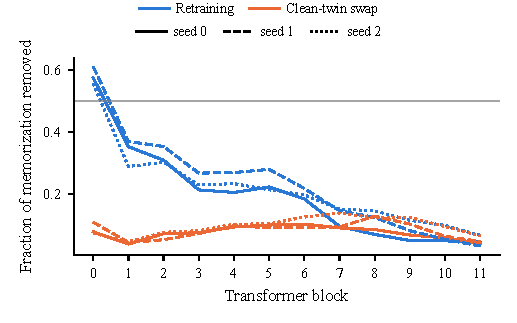
\includegraphics[width=\columnwidth]{figures/paper/fig_f_wronglabel.pdf}
  \caption{Fraction of baseline wrong-label memorization removed by
  retraining or swapping each individual block. Swaps use the
  same-seed clean twin. Line styles distinguish seeds.
  The horizontal line marks the mitigation cutoff. The full criterion
  also requires protection of accuracy.}
  \label{fig:wronglabel-removal}
\end{figure}

